\documentclass[11pt]{article}
\usepackage[review]{acl}
\usepackage{times}
\usepackage{latexsym}
\usepackage[T1]{fontenc}
\usepackage[utf8]{inputenc}
\usepackage{microtype}
\usepackage{inconsolata}
\usepackage{graphicx}
\usepackage{booktabs}
\usepackage{amsmath}
\usepackage{capt-of}
\usepackage[indonesian]{babel}
\usepackage{xurl}

\title{StereoQueerEval: Klasifikasi Ujaran Kebencian terhadap\
Komunitas LGBTQIA+ dengan XLM-RoBERTa dan Qwen3.5-9B}
\author{Penulis Anonim}

\begin{document}
\nolinenumbers
\raggedbottom
\maketitle
\begin{abstract}
% Evidence: Q001,Q002,Q004,B002.
Penelitian ini menyajikan penyelesaian Subtask B StereoQueerEval melalui klasifikasi komentar YouTube berbahasa Inggris, Italia, dan Belanda ke dalam kelas \texttt{no}, \texttt{yes\_implicit}, dan \texttt{yes\_explicit}. Pendekatan utama menggunakan \textit{fine-tuning} Qwen3.5-9B dengan LoRA, menggunakan tiga pilihan bahasa \textit{prompt}. XLM-RoBERTa Base digunakan sebagai pembanding pada pembagian data yang sama. Seluruh pilihan \textit{prompt} Qwen menghasilkan \textit{macro-F1} lebih tinggi daripada pembanding. Skor tertinggi pada pengujian internal adalah 0,719146 pada data Inggris, 0,7036 pada data Italia, dan 0,641522 pada data Belanda. Kesamaan bahasa \textit{prompt} dan komentar belum memberikan hasil tertinggi secara konsisten. Kelas \texttt{yes\_implicit} memperoleh F1 terendah pada kedua model.
\end{abstract}

\section{Pendahuluan}
% Evidence: L102.
Deteksi \textit{hate speech} tidak hanya berkaitan dengan pengenalan kata-kata kasar. Pesan yang menyerang kelompok tertentu juga dapat disampaikan melalui ungkapan tersirat yang membutuhkan pemahaman konteks. \citet{elsherief-etal-2021-latent} menjelaskan bahwa bahasa berkode dan ungkapan tidak langsung menjadi tantangan dalam mendeteksi pesan tersebut. Perbedaan cara penyampaian membuat model perlu mengenali maksud pesan, bukan hanya kata-kata yang muncul di dalamnya.

% Evidence: L111.
Penelitian \citet{chan-etal-2024-hate} mengkaji deteksi \textit{hate speech} terhadap komunitas LGBTQIA+ menggunakan GPT-3.5-turbo pada teks asli dan teks yang diterjemahkan ke bahasa Inggris. Penerjemahan tidak selalu membantu klasifikasi. Analisis kesalahan menunjukkan bahwa istilah \textit{slang} dan ungkapan yang berkaitan dengan budaya tertentu tidak diterjemahkan dengan tepat. Hasil ini menjadi pertimbangan untuk mempertahankan bahasa asli komentar.

% Evidence: L111,Q001,Q006.
Salah satu hal yang belum diuji oleh \citet{chan-etal-2024-hate} adalah penggunaan bahasa \textit{prompt} yang berbeda. Penelitian tersebut menggunakan \textit{prompt} berbahasa Inggris, termasuk untuk data non-Inggris, dan menyarankan pengujian bahasa \textit{prompt} yang sesuai dengan data beserta model lain. Saran ini menjadi dasar penggunaan Qwen dengan \textit{prompt} Inggris, Italia, dan Belanda, baik pada bahasa komentar yang sama maupun berbeda.

% Evidence: L110,L115,Q001,B002.
Penelitian ini berfokus pada penyelesaian \textit{Subtask B: Hate Speech Classification} dalam SemEval-2027 Task 8: StereoQueerEval. Komentar berbahasa Inggris, Italia, dan Belanda diklasifikasikan ke dalam kelas \texttt{no}, \texttt{yes\_implicit}, dan \texttt{yes\_explicit}. XLM-RoBERTa digunakan sebagai \textit{baseline} karena prapelatihan multibahasanya mendukung berbagai tugas pemahaman bahasa lintas bahasa \citep{conneau-etal-2020-unsupervised}. Hasilnya dibandingkan dengan Qwen pada \textit{test} yang sama.

% Evidence: Q001,Q002,Q004,Q006,B002.
Tujuan penelitian ini adalah menyelesaikan klasifikasi dengan membandingkan XLM-RoBERTa dan Qwen melalui sembilan kombinasi bahasa data dan bahasa \textit{prompt}. Tiga versi \textit{prompt} memuat arahan dengan makna yang setara, sementara komentar tetap menggunakan bahasa aslinya. Hasil dianalisis untuk melihat apakah kesamaan bahasa \textit{prompt} dan komentar memberikan skor lebih tinggi, sekaligus mengenali kelas yang masih sulit dibedakan.

\section{Deskripsi \textit{Task}}
% Evidence: L110,L117,Q001.
SemEval-2027 Task 8: StereoQueerEval mengkaji stereotip dan ujaran kebencian terhadap komunitas LGBTQIA+.\footnote{\url{https://semeval.github.io/SemEval2027/tasks.html}} Subtask B meminta klasifikasi komentar ke dalam tiga kelas: \texttt{no} untuk komentar tanpa ujaran kebencian, \nolinkurl{yes_implicit} untuk kebencian yang disampaikan tidak langsung, dan \nolinkurl{yes_explicit} untuk kebencian yang dinyatakan langsung \citep{stereoqueereval-2026-data}. Percobaan menggunakan bahasa Inggris (EN), Italia (IT), dan Belanda (NL). Teks komentar menjadi \textit{input} model, tanpa judul, deskripsi video, atau anotasi dari \textit{subtask} lain.

\subsection{Penelitian Terkait}
% Evidence: L114,L101,L111.
\citet{nozza-2022-nozza} menggabungkan prediksi BERT, RoBERTa, dan HateBERT untuk mengenali homofobia dan transfobia pada komentar YouTube Inggris. QUEEREOTYPES menyediakan anotasi stereotip dan ujaran kebencian secara terpisah pada data Italia \citep{cignarella-etal-2024-queereotypes}. Sementara itu, \citet{chan-etal-2024-hate} menggunakan GPT-3.5-turbo untuk klasifikasi dua kelas dan mengevaluasinya dengan \textit{weighted-F1}. Penelitian ini membedakan tiga kelas menggunakan \textit{macro-F1}, sehingga skornya tidak dibandingkan langsung dengan penelitian tersebut.

% Evidence: L112,L116,Q001,Q006.
\citet{nguyen-etal-2025-leveraging} mengevaluasi lima model bahasa besar pada deteksi ujaran yang menyerang komunitas LGBTQIA+ tanpa pelatihan tambahan dan melaporkan bahwa kesalahan klasifikasi masih terjadi. Penelitian ini menggunakan \textit{fine-tuning} untuk mempelajari kategori StereoQueerEval. Pilihan bahasa \textit{prompt} juga relevan pada model multibahasa. \citet{behzad-etal-2024-ask} menemukan perbedaan hasil antarbahasa \textit{prompt} pada penilaian tata bahasa Inggris. Temuan tersebut menjadi pertimbangan pengujian pilihan bahasa, bukan bukti langsung pada deteksi ujaran kebencian.

\section{Metodologi}
\subsection{XLM-RoBERTa}
% Evidence: L115.
XLM-RoBERTa merupakan model \textit{Transformer} multibahasa yang dilatih menggunakan lebih dari 2 TB teks CommonCrawl dari 100 bahasa \citep{conneau-etal-2020-unsupervised}. Model ini mempelajari hubungan antarkata melalui \textit{masked language modeling}, yaitu memprediksi token yang disembunyikan berdasarkan konteks di sekitarnya. Dengan cara tersebut, satu model dapat membentuk representasi teks dari berbagai bahasa.

XLM-RoBERTa menggunakan arsitektur \textit{encoder} yang membaca konteks dari kedua arah. \textit{Output} model berupa representasi token yang dapat digunakan untuk berbagai tugas pemahaman bahasa, termasuk klasifikasi teks. Varian Base digunakan dalam penelitian ini dan selanjutnya disebut XLM-R.

\subsection{Qwen3.5-9B}
% Evidence: L103.
Qwen3.5-9B adalah model multibahasa dengan sekitar sembilan miliar parameter \citep{qwen-team-2026-qwen35}. Model ini mendukung \textit{input} teks dan visual. Komponen bahasanya menghasilkan teks secara bertahap dengan memperkirakan token berikutnya berdasarkan konteks yang telah tersedia.

Berbeda dari model yang menghasilkan representasi teks untuk lapisan klasifikasi, Qwen dapat menghasilkan \textit{output} teks berdasarkan \textit{prompt}. \textit{Prompt} memberikan konteks dan menjelaskan bentuk \textit{output} yang diharapkan. Kemampuan tersebut memungkinkan model digunakan untuk berbagai tugas bahasa melalui format percakapan.

\subsection{Alur Analisis}
% Evidence: Q001,Q004,Q005,Q006,B002.
Alur analisis meliputi eksplorasi data, prapemrosesan dan pembagian data, pelatihan dan prediksi, kemudian evaluasi. Langkah tersebut diterapkan pada setiap bahasa secara terpisah.

\subsubsection{Eksplorasi Data (EDA)}
% Evidence: Q007.
Eksplorasi data atau \textit{exploratory data analysis} (EDA) memeriksa distribusi kelas, kelengkapan kolom, keunikan ID, dan duplikasi. Hasil pemeriksaan digunakan untuk memahami komposisi data sebelum pembagian.

\subsubsection{Prapemrosesan dan Pembagian Data}
% Evidence: Q005,Q007,L118.
Prapemrosesan menggunakan normalisasi Unicode NFKC untuk menyeragamkan representasi karakter yang setara agar kesamaan teks dapat diperiksa secara konsisten \citep{unicode-consortium-2026-normalization}. Kapitalisasi, emoji, dan tanda baca dipertahankan. Komentar tidak diterjemahkan.

% Evidence: Q005,Q007,Q001,B002.
Pembagian dilakukan per bahasa dengan stratifikasi label dan pengelompokan konteks video, menggunakan \textit{seed} 42. Targetnya 70\% \textit{train}, 10\% \textit{validation}, dan 20\% \textit{test}. Komentar dengan pasangan judul--deskripsi yang sama atau duplikat setelah normalisasi ditempatkan pada kelompok yang sama agar tidak terpisah antarbagian. Komentar kemudian ditokenisasi dan dipotong sesuai batas \textit{input} masing-masing model.

\subsubsection{Pelatihan dan Prediksi}
% Evidence: B002.
XLM-R menggunakan lapisan klasifikasi untuk menghasilkan satu dari tiga label. Seluruh parameter diperbarui selama pelatihan. Bobot kelas dihitung hanya dari \textit{train} untuk memperhatikan kelas dengan contoh lebih sedikit.

% Evidence: Q001,Q004,L104.
Pada Qwen, \textit{fine-tuning} menggunakan \textit{Low-Rank Adaptation} (LoRA) dan \textit{supervised fine-tuning} (SFT). LoRA mempertahankan bobot utama model dan memperbarui parameter tambahan berukuran kecil \citep{hu-etal-2021-lora}. Perhitungan kesalahan hanya dilakukan pada bagian \textit{output}, tanpa menyertakan \textit{prompt} dan komentar.

% Evidence: Q001,Q004,Q006.
\textit{Prompt} menjelaskan tiga kategori dan menegaskan bahwa penyebutan identitas LGBTQIA+ saja tidak cukup untuk menentukan kebencian. Pilihan bahasanya adalah Inggris, Italia, dan Belanda, tanpa contoh komentar berlabel. \textit{Output} dipetakan menjadi angka 0 untuk \texttt{no}, 1 untuk \texttt{yes\_explicit}, dan 2 untuk \texttt{yes\_implicit}. Komentar tetap menggunakan bahasa aslinya, sedangkan nama penanda bahasa dan komentar pada format \textit{input} ditulis dalam bahasa Inggris untuk seluruh pilihan \textit{prompt}.

% Evidence: Q001,Q004.
Saat prediksi, jumlah log probabilitas setiap pilihan \textit{output} beserta penanda akhirnya dihitung. Pilihan dengan skor tertinggi menjadi label prediksi. Cara ini membatasi \textit{output} pada tiga kategori yang ditentukan, sehingga label tidak bergantung pada penjelasan bebas yang dihasilkan model.

\subsubsection{Evaluasi Model}
% Evidence: Q001,Q003,Q004,B002.
Evaluasi pada akhir setiap \textit{epoch} digunakan untuk memilih model dengan \textit{macro-F1} tertinggi pada \textit{validation}. Model terpilih dievaluasi pada \textit{test} yang sama untuk kedua pendekatan. Label yang benar pada \textit{test} hanya digunakan untuk menghitung metrik evaluasi.

\subsection{Metrik Evaluasi}
% Evidence: Q001,Q002,Q003,Q004,B002.
Kinerja model dievaluasi menggunakan \textit{macro-F1} sebagai metrik utama. Metrik ini memberikan bobot yang sama kepada kelas \texttt{no}, \texttt{yes\_implicit}, dan \texttt{yes\_explicit}, sehingga sesuai untuk mengevaluasi kinerja ketika jumlah contoh antarkelas berbeda. \textit{Macro-F1} dihitung sebagai rata-rata F1 ketiga kelas.

F1 merupakan rata-rata harmonik \textit{precision} dan \textit{recall}. \textit{Precision} menyatakan proporsi prediksi suatu kelas yang benar, sedangkan \textit{recall} menyatakan proporsi contoh aktual kelas tersebut yang berhasil dikenali. Perhitungannya dirumuskan sebagai:
\begin{equation}
F1_c = \frac{2P_cR_c}{P_c+R_c},
\end{equation}
\begin{equation}
\text{\textit{Macro-F1}} = \frac{1}{3}\sum_{c=1}^{3}F1_c.
\end{equation}
$P_c$ dan $R_c$ masing-masing menyatakan \textit{precision} dan \textit{recall} kelas $c$. \textit{Macro-F1} pada \textit{validation} digunakan untuk memilih \textit{checkpoint} terbaik, sedangkan kinerja akhir dilaporkan pada \textit{test} untuk setiap bahasa dan konfigurasi eksperimen. F1 per kelas juga disajikan untuk mengidentifikasi kategori yang masih sulit dikenali.

\section{Rancangan Eksperimen}
% Evidence: Q005,Q007,L110.
\textit{Dataset} terdiri atas 7.627 komentar berlabel dari penyelenggara StereoQueerEval. Pengujian menggunakan pembagian internal data tersebut, sehingga hasil belum merupakan evaluasi resmi \textit{shared task}. Judul dan deskripsi hanya digunakan untuk pengelompokan konteks saat pembagian.

% Evidence: Q001,Q002,Q004,Q006,B002.
XLM-R dilatih satu kali per bahasa. Qwen dilatih pada sembilan pasangan bahasa komentar dan bahasa \textit{prompt}, masing-masing dimulai dari model dasar yang sama dengan parameter LoRA baru. Bahasa \textit{prompt} digunakan secara konsisten pada \textit{train}, \textit{validation}, dan \textit{test}. Pelatihan dilakukan menggunakan Python dan PyTorch dengan GPU melalui platform Modal.

% Evidence: Q001,Q004,Q008,B002,L109.
Tabel~\ref{tab:configuration} merangkum konfigurasi kedua model. Keduanya menggunakan AdamW \citep{loshchilov-hutter-2019-decoupled}. Batas \textit{input} Qwen memperhitungkan \textit{prompt}, komentar, dan \textit{output}. Pelatihan berhenti ketika skor \textit{validation} tidak membaik sesuai ketentuan \textit{early stopping}. Untuk pasangan yang diulang, hasil dilaporkan dari percobaan terbaru, tanpa memilih berdasarkan skor \textit{test}.

\begin{table}[t]
\centering\small
\setlength{\tabcolsep}{2.5pt}
\begin{tabular}{lcc}
\toprule
Pengaturan & XLM-R & Qwen \\
\midrule
\textit{Fine-tuning} & Seluruh parameter & SFT LoRA \\
\textit{Seed} & 42 & 42 \\
\textit{Epoch} maksimum & 10 & 5 \\
\textit{Learning rate} & $10^{-5}$ & $10^{-4}$ \\
\textit{Weight decay} & 0,01 & 0,01 \\
\textit{Batch size} & 32 & 16 \\
Batas \textit{input} & 384 token & 1.024 token \\
\textit{Scheduler} & \textit{Linear} & \textit{Cosine} \\
\textit{Warmup} & -- & Sekitar 5\% langkah \\
\textit{Early stopping} & 3 & 2 \\
LoRA \textit{rank}/\textit{alpha} & -- & 16/32 \\
LoRA \textit{dropout} & -- & 0,05 \\
\bottomrule
\end{tabular}
\caption{Konfigurasi pelatihan. \textit{Early stopping} menyatakan jumlah evaluasi tanpa perbaikan pada \textit{validation}.}
\label{tab:configuration}
\end{table}

\section{Hasil dan Pembahasan}
\subsection{Eksplorasi Data (EDA)}
% Evidence: Q007.
Data terdiri atas 2.989 komentar Inggris, 2.400 Italia, dan 2.238 Belanda. Gambar~\ref{fig:eda-labels} menunjukkan bahwa kelas \texttt{no} berjumlah paling banyak dan \texttt{yes\_implicit} paling sedikit pada setiap bahasa. Ketidakseimbangan tersebut mendukung penggunaan \textit{macro-F1} agar setiap kelas mendapat bobot evaluasi yang sama.

\begin{figure*}[t]
\centering
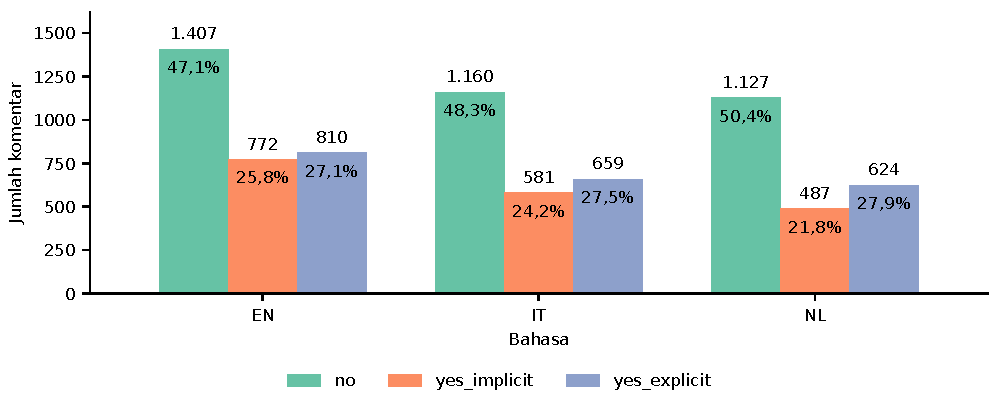
\includegraphics[width=\textwidth]{figures/eda_label_distribution.pdf}
\caption{Distribusi kelas sebelum pembagian. Jumlah komentar ditampilkan di atas batang dan persentase terhadap total per bahasa di dalam batang.}
\label{fig:eda-labels}
\end{figure*}

% Evidence: Q007.
Proporsi \texttt{no} mendekati separuh data, sedangkan \texttt{yes\_implicit} berada pada kisaran 21,76\%--25,83\%. Distribusi label perlu diperhatikan saat membaca F1 per kelas, tetapi belum menjelaskan penyebab perbedaan kinerja antarbahasa.

\subsection{Prapemrosesan dan Pembagian Data}
% Evidence: Q005,Q007,B002.
Pemeriksaan tidak menemukan nilai kosong pada kolom yang dianalisis. Seluruh ID unik dan label sesuai tiga kelas. Satu duplikasi komentar pada data Italia memiliki label yang sama dan berada pada \textit{train}. Seluruh komentar tetap teralokasi tanpa perubahan isi. Tidak ditemukan tumpang tindih ID, komentar ternormalisasi, atau pasangan judul--deskripsi nonkosong antarbagian. Jumlah hasil pembagian disajikan pada Tabel~\ref{tab:split}.

% Evidence: Q005,Q007.
Hasil pembagian mendekati target 70:10:20, dengan jumlah aktual mengikuti kelompok komentar yang dipertahankan bersama. Dengan demikian, rasio tidak dipaksakan tepat apabila memerlukan pemisahan anggota kelompok. Pemeriksaan tumpang tindih membantu memastikan bahwa komentar yang sama tidak muncul pada bagian yang digunakan untuk pelatihan dan pengujian.

\begin{table}[t]
\centering\small
\begin{tabular}{lrrr}
\toprule
Data & \textit{Train} & \textit{Validation} & \textit{Test} \\
\midrule
EN & 2.111 & 292 & 586 \\
IT & 1.699 & 220 & 481 \\
NL & 1.556 & 226 & 456 \\
\bottomrule
\end{tabular}
\caption{Jumlah komentar setelah pembagian. Ketiga kelas hadir pada setiap bagian.}
\label{tab:split}
\end{table}

\subsection{Hasil Klasifikasi Berdasarkan Bahasa}
% Evidence: Q002,B002.
Tabel~\ref{tab:main} membandingkan XLM-R dengan sembilan pasangan bahasa Qwen pada \textit{test} yang sama. Seluruh pilihan \textit{prompt} Qwen memperoleh \textit{macro-F1} lebih tinggi daripada XLM-R.

\begin{table}[t]
\centering\small
\setlength{\tabcolsep}{2pt}
\begin{tabular}{lrrrr}
\toprule
Data & XLM-R & Q-EN & Q-IT & Q-NL \\
\midrule
EN & 0.529052 & \textbf{0.719146} & 0.715757 & 0.688340 \\
IT & 0.574515 & \textbf{0.7036} & 0.694249 & 0.701449 \\
NL & 0.507678 & 0.629927 & 0.630810 & \textbf{0.641522} \\
\bottomrule

\end{tabular}
\caption{\textit{Macro-F1} pada \textit{test}. Q-EN, Q-IT, dan Q-NL adalah Qwen dengan bahasa \textit{prompt} EN, IT, dan NL. Nilai Qwen tertinggi per bahasa dicetak tebal.}
\label{tab:main}
\end{table}

\begin{table*}[t]
\centering\small
\begin{tabular}{lllrrr}
\toprule
Data & Model & \textit{Prompt} & \texttt{no} & \texttt{yes\_implicit} & \texttt{yes\_explicit} \\
\midrule
EN & XLM-R & -- & 0.6569 & 0.4085 & 0.5217 \\
EN & Qwen & EN & \textbf{0.8406} & \textbf{0.6172} & 0.6996 \\
EN & Qwen & IT & 0.8229 & 0.5882 & \textbf{0.7362} \\
EN & Qwen & NL & 0.8250 & 0.5397 & 0.7003 \\
IT & XLM-R & -- & 0.7056 & 0.4747 & 0.5432 \\
IT & Qwen & EN & \textbf{0.7876} & \textbf{0.6127} & 0.7104 \\
IT & Qwen & IT & 0.7786 & 0.5815 & \textbf{0.7227} \\
IT & Qwen & NL & 0.7806 & 0.6020 & 0.7217 \\
NL & XLM-R & -- & 0.6742 & 0.3304 & 0.5185 \\
NL & Qwen & EN & 0.8118 & \textbf{0.5094} & 0.5686 \\
NL & Qwen & IT & 0.7908 & 0.4806 & 0.6210 \\
NL & Qwen & NL & \textbf{0.8140} & 0.4828 & \textbf{0.6278} \\
\bottomrule

\end{tabular}
\caption{F1 setiap kelas pada \textit{test}. Kolom \textit{prompt} hanya berlaku untuk Qwen. Nilai Qwen tertinggi pada setiap kelas dan bahasa data dicetak tebal.}
\label{tab:classes}
\end{table*}

% Evidence: Q002,B002.
Hasil tertinggi disajikan secara deskriptif, bukan sebagai pengaturan akhir yang dipilih melalui \textit{validation}. Perbedaan ukuran model, \textit{tokenizer}, batas \textit{input}, dan pelatihan membuat selisih kedua pendekatan belum dapat dikaitkan dengan satu komponen tertentu.

% Evidence: Q002,B002.
Pada data Inggris, XLM-R memperoleh \textit{macro-F1} sebesar 0,529052. Skor tertinggi Qwen adalah 0,719146, dengan selisih sekitar 0,1901. \textit{Prompt} Italia berada di urutan berikutnya dengan skor 0,715757, sedangkan \textit{prompt} Belanda memperoleh 0,688340. Hasil ini menunjukkan bahwa \textit{prompt} Inggris dan Italia memberikan skor yang berdekatan pada data Inggris.

% Evidence: Q002,B002.
Pada data Italia, XLM-R memperoleh skor 0,574515. Qwen dengan \textit{prompt} Inggris memperoleh 0,7036, diikuti \textit{prompt} Belanda sebesar 0,701449 dan \textit{prompt} Italia sebesar 0,694249. Selisih Qwen tertinggi terhadap XLM-R sekitar 0,1291. Pada data ini, penggunaan bahasa \textit{prompt} yang sama dengan komentar belum memberikan skor tertinggi.

% Evidence: Q002,B002.
Pada data Belanda, XLM-R memperoleh skor 0,507678. Skor Qwen tertinggi adalah 0,641522 dengan \textit{prompt} Belanda, diikuti \textit{prompt} Italia sebesar 0,630810 dan \textit{prompt} Inggris sebesar 0,629927. Selisih tertinggi terhadap XLM-R sekitar 0,1338. Walaupun Qwen melampaui pembanding pada ketiga pilihan, kinerja pada data Belanda tetap lebih rendah daripada dua bahasa lain.

\subsection{Analisis Berdasarkan Kelas}
% Evidence: Q002,B002.
Tabel~\ref{tab:classes} memperlihatkan bahwa \texttt{no} memperoleh F1 tertinggi dan \texttt{yes\_implicit} terendah pada setiap pengaturan kedua model. Seluruh pilihan \textit{prompt} Qwen menghasilkan F1 lebih tinggi daripada XLM-R untuk ketiga kelas pada bahasa data yang sama.



% Evidence: Q002.
Pada data Inggris dan Italia, \textit{prompt} Inggris memberikan F1 tertinggi untuk \texttt{no} dan \nolinkurl{yes_implicit}, sedangkan \textit{prompt} Italia tertinggi untuk \nolinkurl{yes_explicit}. Pada data Belanda, \textit{prompt} Belanda tertinggi untuk \texttt{no} dan \nolinkurl{yes_explicit}, tetapi \textit{prompt} Inggris tertinggi untuk \nolinkurl{yes_implicit}. Dengan demikian, \textit{prompt} dengan \textit{macro-F1} tertinggi belum tentu terbaik pada setiap kelas.

% Evidence: Q002.
Pada kelas \texttt{yes\_implicit}, F1 Qwen berada pada rentang 0,5397--0,6172 untuk data Inggris, 0,5815--0,6127 untuk data Italia, dan 0,4806--0,5094 untuk data Belanda. Bahkan pilihan \textit{prompt} tertinggi pada kelas tersebut masih menghasilkan skor lebih rendah daripada dua kelas lainnya dalam pengaturan yang sama. Perbaikan klasifikasi perlu memberi perhatian pada pembedaan kategori ini, dengan pemeriksaan contoh prediksi untuk mengetahui bentuk kesalahan yang terjadi.

% Evidence: Q002,B002.
F1 XLM-R pada kelas \texttt{yes\_implicit} adalah 0,4085 pada data Inggris, 0,4747 pada data Italia, dan 0,3304 pada data Belanda. Seluruh pilihan Qwen memperoleh F1 lebih tinggi, tetapi kategori ini tetap memiliki skor terendah. Nilai F1 belum menunjukkan kelas tujuan kesalahan, sehingga pola kekeliruan perlu diperiksa langsung pada prediksi.

\section{Kesimpulan}
% Evidence: Q001,Q002,Q004,B002.
Penyelesaian Subtask B StereoQueerEval menggunakan SFT LoRA pada Qwen3.5-9B menghasilkan skor lebih tinggi daripada XLM-R pada pengujian internal. Skor tertinggi adalah 0,719146 pada data Inggris, 0,7036 pada data Italia, dan 0,641522 pada data Belanda. Kesamaan bahasa \textit{prompt} dan komentar belum konsisten memberikan hasil tertinggi. Pengembangan berikutnya perlu memperkuat klasifikasi \texttt{yes\_implicit} dan memilih pengaturan melalui \textit{validation}.

\section*{Keterbatasan}
% Evidence: Q001,Q004,Q005,Q006,Q007,Q008,B002,L110,L119.
Hasil berasal dari pengujian internal dengan satu \textit{seed} dan satu versi \textit{prompt} per bahasa, sehingga belum menunjukkan kinerja pada \textit{test} resmi atau kestabilan antarpengulangan. Setiap pasangan Qwen melatih \textit{adapter} terpisah, sehingga perbedaan skor tidak hanya menggambarkan bahasa \textit{prompt}. Reproduksibilitas Qwen memerlukan kesamaan model, data, dan konfigurasi perangkat lunak. Kesamaan \textit{seed} belum menjamin hasil identik lintas lingkungan komputasi \citep{pytorch-reproducibility}.

% Daftar pustaka berada di luar batas lima halaman isi dan keterbatasan.
\clearpage
\bibliography{references}
\end{document}
